%!TeX spellcheck = en-CA
%Development of this version is against texlive2024
\RequirePackage[l2tabu, orthodox]{nag}
\documentclass[margin1,line,canadian]{resume}
\usepackage[hyphens]{url}
\usepackage[colorlinks,hypertexnames=false,breaklinks,bookmarks]{hyperref}
\usepackage[canadian]{babel}
\usepackage[activate=true,tracking=true,kerning=true,expansion=true,spacing=true]{microtype}
\microtypecontext{spacing=nonfrench}
\usepackage{booktabs} %makes tables look better
\usepackage[T1]{fontenc} %upgrades font encodings
\usepackage[utf8]{inputenc}%Tells latex the file is saved as UTF-8 (make sure it is!)
\usepackage{lmodern} % To switch to Latin Modern
%\usepackage{ragged2e}
\usepackage{slantsc}
\usepackage{upgreek} %Provides upright (non italic) greek fonts
\usepackage{gensymb} %Provides  \de­gree, \cel­sius, \pert­hou­sand, \mi­cro and \ohm amongst others
\usepackage{textcomp} %Supports lmodern
\usepackage{textgreek} %Provides \textbeta and similar greek letters in text mode
\usepackage{ellipsis}%Fix \ldots and similar commands, bugs with spacing and such
%\usepackage{showframe}
\usepackage[letterpaper,top=0.4in,bottom=0.4in,left=0.4in,right=1.5in,nohead,nomarginpar,includefoot]{geometry}
\usepackage{pageslts}
\usepackage{fancyhdr}
\usepackage{datetime}
\usepackage{tikz}
\usetikzlibrary{backgrounds,calc}
\usepackage{csquotes}
\usepackage{fontawesome}
\usepackage[backend=biber,style=verbose,backref=true,maxnames=99,alldates=iso,seconds=true,bibencoding=utf8,dashed=false,giveninits=true]{biblatex}
\usepackage{etoolbox}
\pagenumbering{arabic}

% https://tex.stackexchange.com/questions/73136/make-specific-author-bold-using-biblatex/416416#416416
% Code to bold my name in citations
\makeatletter
\def\nhblx@bibfile@name{\jobname -nhblx.bib}
\newwrite\nhblx@bibfile
\immediate\openout\nhblx@bibfile=\nhblx@bibfile@name

\immediate\write\nhblx@bibfile{%
  @comment{Auto-generated file}\blx@nl}

\newcounter{nhblx@name}
\setcounter{nhblx@name}{0}

\newcommand*{\nhblx@writenametobib}[1]{%
  \stepcounter{nhblx@name}%
  \edef\nhblx@tmp@nocite{%
    \noexpand\AfterPreamble{%
      \noexpand\setbox0\noexpand\vbox{%
        \noexpand\nhblx@getmethehash{nhblx@name@\the\value{nhblx@name}}}}%
  }%
  \nhblx@tmp@nocite
  \immediate\write\nhblx@bibfile{%
    @misc{nhblx@name@\the\value{nhblx@name}, author = {\unexpanded{#1}}, %
          options = {dataonly=true},}%
  }%
}

\AtEndDocument{%
  \closeout\nhblx@bibfile}

\addbibresource{\nhblx@bibfile@name}

\newcommand*{\nhblx@boldhashes}{}
\DeclareNameFormat{nhblx@hashextract}{%
  \xifinlist{\thefield{hash}}{\nhblx@boldhashes}
    {}
    {\listxadd{\nhblx@boldhashes}{\thefield{hash}}}}

\DeclareCiteCommand{\nhblx@getmethehash}
  {}
  {\printnames[nhblx@hashextract][1-999]{author}}
  {}
  {}

\newcommand*{\addboldnames}{\forcsvlist\nhblx@writenametobib}
\newcommand*{\resetboldnames}{\def\nhblx@boldhashes{}}

\newcommand*{\ifhashinboldlist}{%
  \xifinlist{\thefield{hash}}{\nhblx@boldhashes}}
\makeatother

\newcommand*{\mkboldifhashinlist}[1]{%
  \ifhashinboldlist
    {\mkbibbold{#1}}
    {#1}}

\DeclareNameWrapperFormat{boldifhashinlist}{%
  \renewcommand*{\mkbibcompletename}{\mkboldifhashinlist}%
  #1}

\DeclareNameWrapperAlias{sortname}{default}
\DeclareNameWrapperAlias{default}{boldifhashinlist}
\addboldnames{{Devenyi, G. A.},{Devenyi, Gabriel Allan},{Devenyi, Gabriel},{Devenyi, G A},{Gabriel Devenyi},{Devenyi, GA},{Devenyi, Gabriel A}}
%%%%%%%%%%%%%%%%%%%%%%%%%%%%%%%%%%%%%%%%%%%%%%%%%%%%%%%%%%%%%%%%%%%%%%%


% https://tex.stackexchange.com/questions/341313/biblatex-always-show-a-specific-author/343221?noredirect=1#comment1796361_343221

\newcounter{namesnotimportant}
\newtoggle{ellipsis}

\makeatletter
\newbibmacro*{name:etal:delim}[1]{%
  \ifnumgreater{\value{listcount}}{\value{liststart}}
    {\ifboolexpr{
       test {\ifnumless{\value{listcount}}{\value{liststop}}}
       or
       test \ifmorenames
       or test {\ifnumcomp{\value{namesnotimportant}}{>}{0}}
     }
       {\printdelim{multinamedelim}}
       {\lbx@finalnamedelim{#1}}}
    {}}
\makeatother

\DeclareNameFormat{given-family-etal}{%
  \letbibmacro{name:delim}{name:etal:delim}%
  \ifnumcomp{\value{listcount}}{=}{1}
    {\setcounter{namesnotimportant}{0}%
     \global\toggletrue{ellipsis}}
    {}%
  \ifboolexpr{test {\ifnumcomp{\value{listcount}}{=}{1}}
              or test {\ifnumcomp{\value{listtotal}}{=}{2}}
              or test {\ifnumcomp{\value{listcount}}{=}{\value{listtotal}}}}
    {\ifgiveninits
      {\usebibmacro{name:given-family}
         {\namepartfamily}
         {\namepartgiveni}
         {\namepartprefix}
         {\namepartsuffix}}
      {\usebibmacro{name:given-family}
         {\namepartfamily}
         {\namepartgiven}
         {\namepartprefix}
         {\namepartsuffix}}}%
    {\ifboolexpr{test {\iffieldequalstr{hash}{9eca3b2c038ea2887161409590d86c7e}}
                 or
                 test {\iffieldequalstr{hash}{bbe6f69e72a9242bc1bd6610fee4d49b}}
                 or
                 test {\iffieldequalstr{hash}{d4fc4ad945020d3ec9c3c8c3c4f53a41}}
                 or
                 test {\iffieldequalstr{hash}{e0529bf51d94c9b9e9a2f938046591a0}}
                 or
                 test {\iffieldequalstr{hash}{e323f1f7a8d1e3eafe0590841ea626e2}}}%% <----- put the correct hash here
      {\global\toggletrue{ellipsis}%
       \ifgiveninits
        {\usebibmacro{name:given-family}
           {\namepartfamily}
           {\namepartgiveni}
           {\namepartprefix}
           {\namepartsuffix}}
        {\usebibmacro{name:given-family}
           {\namepartfamily}
           {\namepartgiven}
           {\namepartprefix}
           {\namepartsuffix}}}%
      {\stepcounter{namesnotimportant}%
       \iftoggle{ellipsis}
         {\addcomma\space\textellipsis\global\togglefalse{ellipsis}\isdot}
         {}}}%
  \ifboolexpr{
    test {\ifnumequal{\value{listcount}}{\value{liststop}}}
    and
    (test \ifmorenames
     or test {\ifnumcomp{\value{namesnotimportant}}{>}{0}})
  }
    {\andothersdelim\bibstring{andothers}}
    {}}

\DeclareNameAlias{sortname}{given-family-etal}
\DeclareNameAlias{author}{given-family-etal}
\DeclareNameAlias{editor}{given-family-etal}
\DeclareNameAlias{translator}{given-family-etal}
%%%%%%%%%%%%%%%%%%%%%%%%%%%%%%%%%%%%%%%%%%%%%%%%%%%%%%%%%%%%%%%%%%%%%%%%%%%%%%%%%%%%%%%%%%%%%%%%%%%%%%%%%%%%%%%%%%%%%%%%%%%

\renewcommand{\dateseparator}{-}
\newcommand{\todayiso}{\the\year \dateseparator \twodigit\month \dateseparator \twodigit\day}

%Print url or eprint only if no DOI
\DeclareSourcemap{
 \maps[datatype=bibtex]{
  \map[overwrite]{
   \step[fieldsource=doi, final]
   \step[fieldset=url, null]
   \step[fieldset=eprint, null]
  }
  \map{
   \pertype{article}
   \step[fieldset=issn, null]
  }
 }
}

%Hide ISSN
%\AtEveryBibitem{\ifentrytype{article}{\clearfield{issn}}{}}

%Create a new sorting scheme for biblatex based on ISO year descending
% https://tex.stackexchange.com/questions/46868/biblatex-sorting-by-date
\DeclareSortingScheme{ymdnt}{
 \sort{
  \field{presort}
 }
 \sort[final]{
  \field{sortkey}
 }
 \sort[direction=descending]{ % Change if descending desired
  \field{sortyear}
  \field{year}
 }
 \sort[direction=descending]{
  \field[padside=left,padwidth=2,padchar=0]{month}
  \literal{00}
 }
 \sort[direction=descending]{
  \field[padside=left,padwidth=2,padchar=0]{day}
  \literal{00}
 }
 \sort{
  \field{sortname}
  \field{author}
  \field{editor}
  \field{translator}
  \field{sorttitle}
  \field{title}
 }
 \sort{
  \field{sorttitle}
 }
 \sort{
  \field[padside=left,padwidth=4,padchar=0]{volume}
  \literal{0000}
 }
}

%Headers and footers
\fancyhead{}
\renewcommand{\headrulewidth}{0pt}
\fancyfootoffset[L]{1.085in}
\lfoot{\todayiso}
\cfoot{Gabriel A. Devenyi --- \href{mailto:gabriel.devenyi@mcgill.ca}{gabriel.devenyi@mcgill.ca}}
\rfoot{\thepage\ of \lastpageref{LastPage}}
\pagestyle{fancy}

%Setup PDF file links etc
\hypersetup{
 unicode=true,          % non-Latin characters in Acrobat’s bookmarks
 pdfencoding=unicode,
 pdftoolbar=false,        % show Acrobat’s toolbar?
 pdfmenubar=true,        % show Acrobat’s menu?
 pdffitwindow=true,     % window fit to page when opened
 pdfstartview={FitH},    % fits the width of the page to the window
 pdftitle={\today{} Gabriel A. Devenyi -- Curriculum Vit\ae},    % title
 pdfauthor={Gabriel A. Devenyi},     % author
 pdfsubject={\today{} Gabriel A. Devenyi -- Curriculum Vit\ae},   % subject of the document
 pdfkeywords={neuroimaging} {mri} {segmentation} {structural imaging}, % list of keywords
 pdfnewwindow=true,      % links in new window
 colorlinks=true,       % false: boxed links; true: colored links
 linkcolor=black,          % color of internal links
 citecolor=black,        % color of links to bibliography
 filecolor=black,      % color of file links
 urlcolor=blue           % color of external links
}

\widowpenalty=10000 %Prevent widows (single sentences at end of page)
\clubpenalty=10000 %Prevent orphans (single sentences on empty pages)

%\special{pdf:minorversion 7}
%\special{pdf:objcompresslevel 3}
%\special{pdf:compresslevel 9}
\pdfminorversion=7
\pdfobjcompresslevel=9
\pdfcompresslevel=9

%Actual start of document
\title{Curriculum Vit\ae}
\author{Gabriel A. Devenyi}
\date{\today}

\begin{document}
%Embed a picture in the page of me, top right
\begin{tikzpicture}[remember picture, overlay]
 \begin{pgfonlayer}{background}
  \node [anchor=north east,outer sep=0pt,inner sep=0pt]  at ($(current page.north east) +(-1.5in,-0.4in)$)
  {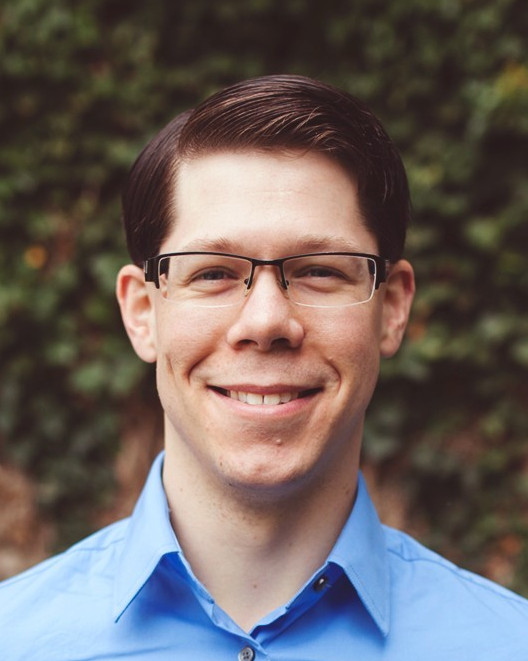
\includegraphics[height=4cm]{headshot}};
 \end{pgfonlayer}
\end{tikzpicture}
\name{\huge Gabriel A. Devenyi}
\begin{resume}
 \section{\mysidestyle{}Professional\\Contact}
 Research Computing Associate\\
 Computational Brain Anatomy (CoBrA) Laboratory \& Cerebral Imaging Center\\
 Project Lead --- Douglas Neuroinformatics Platform\\
 Douglas Mental Health University Institute\\
 \\
 Affiliate Member, Department of Psychiatry\\
 McGill University\\
 \\
 6875 LaSalle Boulevard \hfill \faPhone~514.761.6131$\times$4781\\
 CIC Pavillion, GH-2111 \hfill \faEnvelope~\href{mailto:gabriel.devenyi@mcgill.ca}{gabriel.devenyi@mcgill.ca}\\
 Montr\'{e}al, Qu\'{e}bec \hfill \faGithub~\href{https://github.com/gdevenyi}{gdevenyi}\\
 H4H 1R3, Canada \hfill \faTwitter~\href{https://twitter.com/gadevenyi}{gadevenyi}\\
 \vspace{-4.5mm}%

 \section{\mysidestyle{}Research\\Interests}

 Structural neuroimaging. Image processing, classification, and registration. Pipeline design and optimization
 for standardized image processing. High performance computing. Statistical methods in Neuroimaging.
 Architectural design of data management databases for data capture and management.

 \section{\mysidestyle{}Education}

 \textbf{McMaster University}, Hamilton, ON, Canada\\\vspace{2mm}%
 \textsl{Doctor of Philosophy --- Engineering Physics} \hfill \textbf{2014-06}\vspace{-3mm}\\\vspace{-1mm}%
 \begin{list2}
  \item Thesis : An Investigation into the Role of Energy and Symmetry at Epitaxial Interfaces
  \item Adviser : Dr.~John S. Preston
 \end{list2}\vspace{-1.5mm}
 \textsl{Bachelor of Engineering --- Engineering Physics} \hfill \textbf{2007-05}\vspace{-3mm}\\\vspace{-1mm}
 \begin{list2}
  \item Awarded with Distinction
 \end{list2}

 \section{\mysidestyle{}Honours and\\Awards}
 Canadian Open Neuroscience Platform Research Scholar --- \$50,000 \hfill \textbf{2019}\\
 Nano Ontario Conference Best Poster \hfill \textbf{2011-10}\\%
 McMaster Materials Science \& Engineering Graduate Conference Best Presentation Delivery \hfill \textbf{2010-09}\\%
 NSERC Postgraduate Scholarship D3 --- \$63,000 \hfill \textbf{2009--2011}\\%
 Ontario Graduate Scholarship --- Doctoral --- \$15,000 --- \textsl{Declined} \hfill \textbf{2009} \\%
 Ontario Graduate Scholarship --- Masters --- \$15,000 \hfill \textbf{2008}

 \section{\mysidestyle{}Teaching\\Experience}
 \textbf{Douglas University Mental Health Institute, CIC}, Montreal, QC, Canada \\%
 \textsl{Research Computing Associate --- CIC Software Seminar Series} \hfill \textbf{2014-08 -- Present}

 \textbf{Software Carpentry}, Online\\%
 \textsl{Volunteer Instructor} \hfill \textbf{2012-11 -- Present}

 \vspace{-2mm}
 \textbf{McMaster University}, Hamilton, ON, Canada \\%
 \textsl{Instructor --- MATLS 1M03, Introduction to Materials Science} \hfill \textbf{2014-06 -- 2014-08}\\
 \textsl{Instructor --- ENG PHYS 2CE4, Computational Methods for Engineering Physics} \hfill \textbf{2014-01 -- 2014-04}\\
 \textsl{Teaching Assistant --- ENG PHYS 3F04 Introduction to Solid State} \hfill \textbf{2012-09 -- 2012-12}\\
 \textsl{Teaching Assistant --- ENG PHYS 4A06 Senior Undergraduate Thesis Project} \hfill  \textbf{2008-09 -- 2012-05}\\
 \textsl{Teaching Assistant --- ENG PHYS 4U04 Advanced Computer Laboratories} \hfill \textbf{2008-09 -- 2009-05}

 \section{\mysidestyle{}Research\\Experience}
 \textbf{McMaster University}, Hamilton, ON, Canada\\%
 \textsl{Laboratory Manager} \hfill \textbf{2009-05 -- 2014-05}\\
 \textsl{Summer and Co-op Student Supervisor} \hfill \textbf{2009-09 -- 2014-05}

\section{\mysidestyle{}Journal\\Reviews}
MIT Press \textsl{Imaging Neuroscience} \hfill \textbf{2023}\\
Wiley \textsl{Human Brain Mapping} \hfill \textbf{2022,2023}\\
Organization for Human Brain Mapping \textsl{Aperture Neuro} \hfill \textbf{2021}\\
Springer Nature \textsl{Anatomy and Embryology} \hfill \textbf{2021}\\
Springer Nature \textsl{Brain Structure \& Function} \hfill \textbf{2021}\\
Elsevier \textsl{NeuroImage} \hfill \textbf{2021}\\
Elsevier \textsl{Progress in Neuro-Psychopharmacology \& Biological Psychiatry} \hfill \textbf{2020}\\
PLOS \textsl{ONE} \hfill \textbf{2019}\\
Nature \textsl{Scientific Data} \hfill \textbf{2018}\\
Elsevier \textsl{Applied Surface Science} \hfill \textbf{2015}\\
SPIE \textsl{Journal of Photonics For Energy} \hfill \textbf{2014}

\section{\mysidestyle{}Service}
\textbf{Centre de la Petite Enfance Funville}, Verdun, QC, Canada\\%
\textsl{Board Member} \hfill \textbf{2019-05 -- 2021-05}

\textbf{Software Carpentry}, Online\\%
\textsl{Maintainer and Developer shell-novice Lesson} \hfill \textbf{2014-11 -- 2022-08}

\textbf{McMaster University}, Hamilton, ON, Canada\\%
\textsl{Ex-Officio Member - Engineering Physics Graduate Advisory Committee} \hfill \textbf{2013-12 -- 2014-08}\\
\textsl{Engineering Physics Professorial Search Committee} \hfill \textbf{2010-11 -- 2011-01}\\
\textsl{NanoGiga 2009, 14th Canadian Semiconductor Technology Conference} \hfill \textbf{2009-08}\\
\textsl{Graduate Student Association --- Phoenix Executive Committee} \hfill \textbf{2009-09 -- 2013-12}

\textbf{Nano Ontario}, ON, Canada\\%
\textsl{Board Member At-Large - Chair, Communications Committee} \hfill \textbf{2013-03 -- 2015-01}

\section{\mysidestyle{}Software}
\textbf{\href{https://github.com/CoBrALab/optimized_antsMultivariateTemplateConstruction}{\color{black}optimized\_antsMultivariateTemplateConstruction}}\\%
An automated pipeline to perform multi-level deformation based morphometry (DBM) on brain volume differences for animal and human MRI.\\
GitHub: 22 \faStar{} 8 \faCodeFork

\textbf{\href{https://github.com/gdevenyi/NeuroAnsible}{\color{black}NeuroAnsible}}\\%
An automated deployment tool for transforming an Ubuntu desktop into a neuroimaging workstation in a single step.\\
GitHub: 21 \faStar{} 0 \faCodeFork

\textbf{\href{https://github.com/CoBrALab/iterativeN3}{\color{black}iterativeN3}}\\%
A comprehensive preprocessing (inhomogeneity correction, denoising, field-of-view cropping, and background removal), N-tissue
classification, brain extraction, and standard space alignment tool for human T1-weighted MRIs.\\
GitHub: 0 \faStar{} 0 \faCodeFork

\textbf{\href{https://github.com/CoBrALab/qbatch}{\color{black}qbatch}}\\%
A python cluster abstraction tool for performing command-line based parallelization for SGE, SLURM, LSF and PBS cluster systems.\\
GitHub: 27 \faStar{} 13 \faCodeFork

\section{\mysidestyle{}Bibliometrics}
Peer-Reviewed Articles : 92 (4 first author, 2 senior author)\\
Presentations and Posters in Conference Proceedings : 87\\
Invited Presentations : 11\\
h-index : 31\\
i10-index : 70

 \section{\mysidestyle{}Patents}
 \begin{refsection}[patents.bib]
  \interlinepenalty=10000 %Prevent breaking of paragraphs
  \newrefcontext[sorting=ymdnt]
  \nocite{*}
  \printbibliography[heading=none]
 \end{refsection}
 \section{\mysidestyle{}Invited\\Presentations}
 \begin{refsection}[invited.bib]
  \interlinepenalty=10000 %Prevent breaking of paragraphs
  \newrefcontext[sorting=ymdnt]
  \nocite{*}
  \printbibliography[heading=none]
 \end{refsection}
 \section{\mysidestyle{}Contributed\\Publications}
 \begin{refsection}[contributed.bib]
  \interlinepenalty=10000 %Prevent breaking of paragraphs
  \newrefcontext[sorting=ymdnt]
  \nocite{*}
  \printbibliography[heading=none]
 \end{refsection}
 \section{\mysidestyle{}Peer-Reviewed\\Publications}
 \begin{refsection}[papers.bib]
  \interlinepenalty=10000 %Prevent breaking of paragraphs
  \newrefcontext[sorting=ymdnt]
  \nocite{*}
  \printbibliography[heading=none]
 \end{refsection}

\end{resume}
\end{document}
